\title{Assignment 3: Intro to Web-Based Interaction}
\author{
        %\large
        \textsc{Caitlin Ross}
  %          \qquad
     %   \textsc{}
        \mbox{}\\ %
        Department of Computer Science\\
        CSCI 6963\\
       %  \\
       % \mbox{}\\ %
        \normalsize
            \texttt{rossc3}
        \normalsize
            \texttt{@rpi.edu}
}
\date{\today}
\documentclass[11pt]{article}
%\documentclass{acmconf}

\usepackage[letterpaper,dvips,top=1.5cm,left=1.5cm,right=1.5cm,
    foot=1cm,bottom=1.5cm]{geometry}
%\usepackage[letterpaper, portrait, margin=2in]{geometry}
%\usepackage[a4paper,showframe=true,bindingoffset=0.2in,%
  %          left=1in,right=1in,top=1in,bottom=1in,%
   %         footskip=.25in]{geometry}

\usepackage{times}
%\usepackage{graphicx}
\usepackage[fleqn]{amsmath}
\usepackage{amsfonts}
\usepackage{amssymb}
\usepackage{amsthm}
\usepackage{amsopn}
\usepackage{xspace}
\usepackage{array}
\usepackage{epsfig}
\usepackage{url}
\usepackage{color}

\numberwithin{figure}{section}

\newcommand\CC{\Lang{\mbox{C++}}\xspace}
\newcommand\Lang[1]{\textsc{#1}}
\newcommand{\kw}[1]{\texttt{\textbf{#1}}}
\newcommand{\cd}[1]{\texttt{#1}}

\newcommand\Naturals{\ensuremath{\mathbb{N}}\xspace}
\newcommand\Integers{\ensuremath{\mathbb{Z}}\xspace}
\newcommand\Rationals{\ensuremath{\mathbb{Q}}\xspace}
\newcommand\Reals{\ensuremath{\mathbb{R}}\xspace}
\newcommand\Complex{\ensuremath{\mathbb{C}}\xspace}

\newcommand\norm[1]{\ensuremath{\lVert#1\rVert}}
\newcommand\abs[1]{\ensuremath{\lvert#1\rvert}}
\newcommand\ceil[1]{\ensuremath{\lceil#1\rceil}}
\newcommand\floor[1]{\ensuremath{\lfloor#1\rfloor}}
\newcommand\set[1]{\ensuremath{\{#1\}}}
\newcommand\angular[1]{\ensuremath{\langle#1\rangle}}

\newcommand\Norm[1]{\ensuremath{\left\lVert#1\right\rVert}}
\newcommand\Abs[1]{\ensuremath{\left\lvert#1\right\rvert}}
\newcommand\Ceil[1]{\ensuremath{\left\lceil#1\right\rceil}}
\newcommand\Floor[1]{\ensuremath{\left\lfloor#1\right\rfloor}}
\newcommand\Set[1]{\ensuremath{\left\{#1\right\}}}
\newcommand\Angular[1]{\ensuremath{\left\langle#1\right\rangle}}

\newcommand{\LOOM}{\ensuremath{\cal{LOOM}}\xspace}
\newcommand{\PolyTOIL}{\textbf{PolyTOIL}\xspace}

\newtheorem{theorem}{Theorem}[section]
\newtheorem{definition}[theorem]{Definition}
\newtheorem{lemma}[theorem]{Lemma}
\newtheorem{corollary}[theorem]{Corollary}
\newtheorem{fact}[theorem]{Fact}
\newtheorem{example}[theorem]{Example}

\newcommand\Cls[1]{\textsf{#1}}
\newcommand\Fig[1]{Figure~\ref{Figure:#1}}

\usepackage{labels} %
%\usepackage{equation}
%\usepackage{prog2tex}

\newenvironment{excerpt}{\begin{quote}\begin{minipage}\textwidth}{\end{minipage}\end{quote}}

\setcounter{topnumber}{0}
\setcounter{bottomnumber}{0}
\setcounter{totalnumber}{20}
\renewcommand{\textfraction}{0.01}

\begin{document}
\newgeometry{margin=1in}
\maketitle
\section{Introduction}
The purpose of this assignment is to use D3: Data-Driven Documents\footnote{http://www.d3js.org} to create interactive visualizations.  After exploring examples on the D3 website, I chose a calendar example to modify in order to show time series data from my research simulations.  This write up discusses the ideas for the visualization.  This includes some storyboard sketches that I drew before writing the code. Then I discuss the Javascript written for this visualization and provide a review of my experience using D3.  At the end, I also discuss some future plans for better implementing this visualization into my work.

\section{Design}
When first looking at examples on the D3 website, I came across a calendar example by Mike Bostock\footnote{http://bl.ocks.org/mbostock/4063318} that I really liked.  The example uses this design to visualize Dow Jones Historical data.  I realized that this would be a good way to view how some metrics measured during my simulations change over simulated time.  My simulation looks at how jobs (which are broken up into tasks) are scheduled at clients at two wide area network sites.  There are four possible scheduling policies.  For my visualization, I chose 3 metrics to look at: client utilization, job response time, and data movement overhead.  

\color{red}TODO: Add storyboard pictures\color{black}


%\begin{figure}[ht]
%	\centering
%		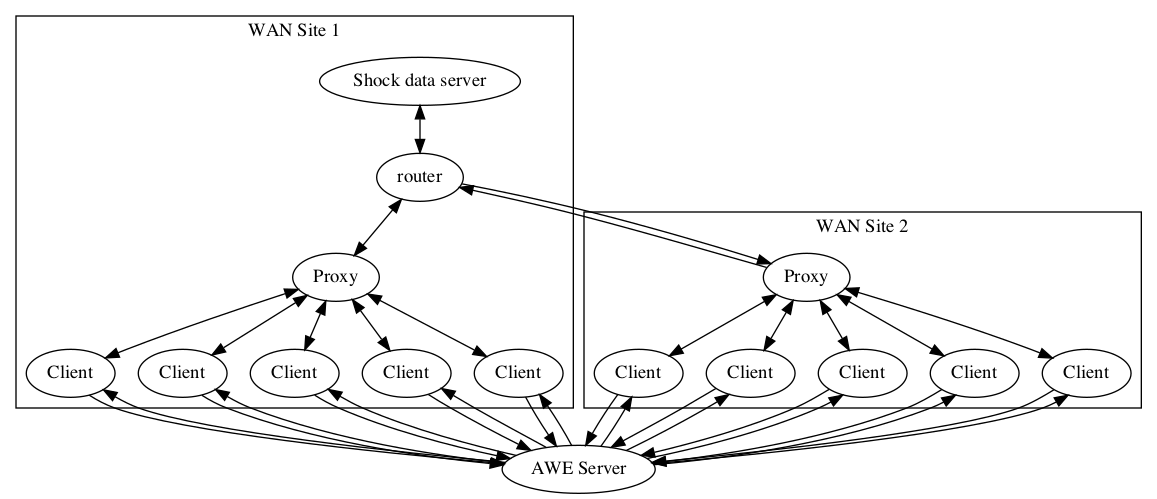
\includegraphics[width=6in]{awesim.png}
%	\caption{MG-RAST infrastructure drawn with GraphViz}
%	\label{fig:awesim}
%\end{figure}

\section{Implementation}
I started with the code provided for the calendar example and adapted that to my needs.  The code sets up an 11 color heat map.  Lower values are more blue and larger values are more red.  Several scalable vector graphics (SVG) objects are created in order to create the parts of the visualization.  There is one SVG for each site, as well as the key.  Below the key there are drop down boxes that allow the scheduling policy and metric to be chosen for viewing.  Upon new selections in either box, a \texttt{loadData()} function is called that loads the appropriate CSV file (there's one file for each scheduling policy) or chooses which metric to pull from the given CSV file.  Currently the visualization is using data generated randomly (though somewhat loosely based on patterns I expect to see).  

I placed my code on my RPI website, which can be found at: \url{http://homepages.rpi.edu/~rossc3/vis.html}. Figure \ref{fig:begin} shows the website when it is first loaded.  At the bottom are brief explanations of the various scheduling policies and metrics used in my work.  Each block represents a day of simulated time and the days are organized into to weeks.  When clicking on the scheduling policy and/or metric boxes, the visualization updates appropriately.  For example, Figure \ref{fig:greedy} shows the visualization after choosing the Greedy scheduling policy and client utilization metric, while Figure \ref{fig:job} shows the data for job response time for FCFS scheduling.  In Figure \ref{fig:greedy}, it is easy to see that on average, the clients tend to have a much higher utilization at the remote site, while local site clients are fairly underutilized.  Note that for Figure \ref{fig:job} there is only one site.  This is because job response time is measured for the whole system (since for most scheduling policies, tasks from the same job can be computed at different sites), so for this metric, the bottom site gets hidden and the label changed to show that it represents the full system.

\begin{figure}[ht]
	\centering
		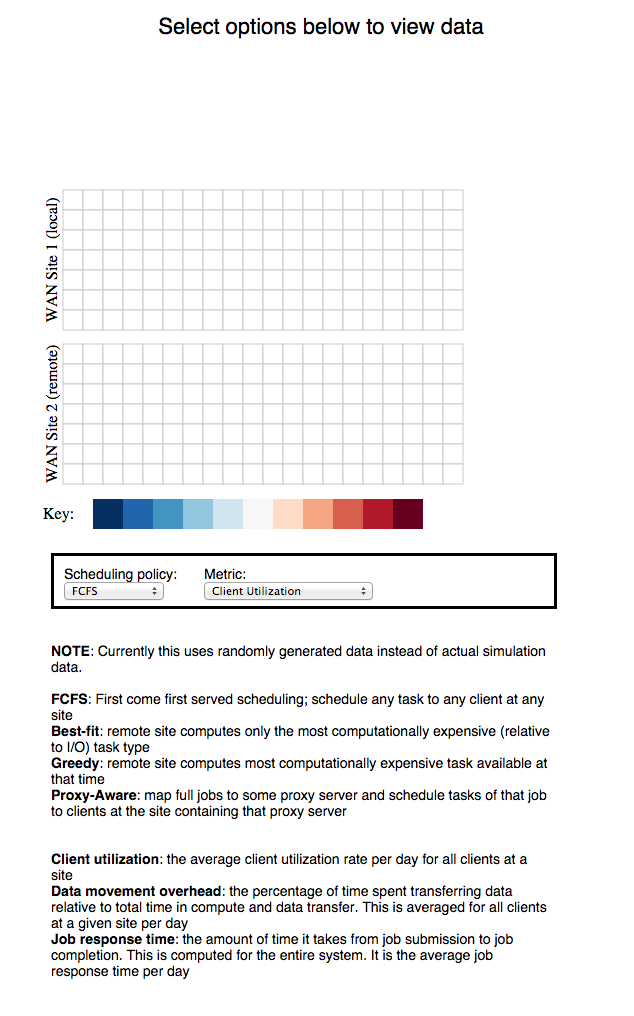
\includegraphics[width=5in]{fig1.png}
	\caption{D3 Visualization when first loaded on webpage}
	\label{fig:begin}
\end{figure}

\begin{figure}[ht]
	\centering
		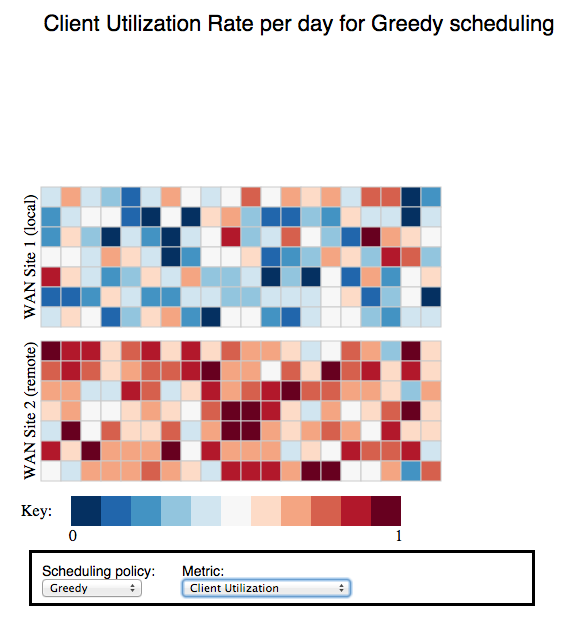
\includegraphics[width=5in]{fig2.png}
	\caption{D3 Visualization after choosing Greedy Scheduling and Client Utilization}
	\label{fig:greedy}
\end{figure}

\begin{figure}[ht]
	\centering
		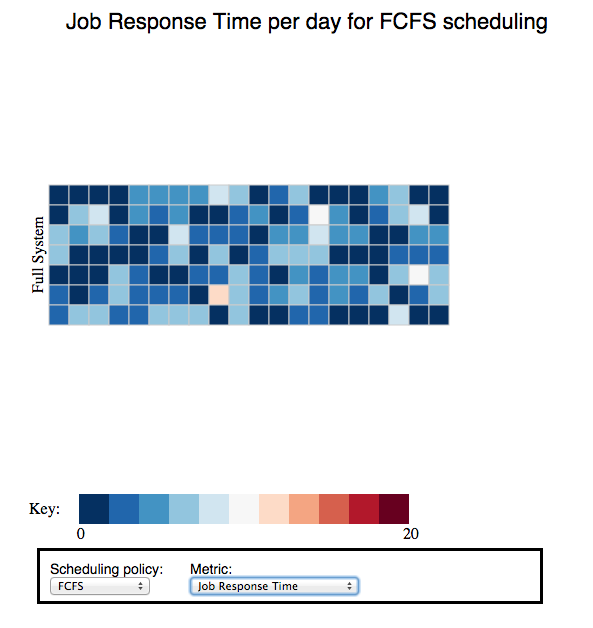
\includegraphics[width=5in]{fig3.png}
	\caption{D3 Visualization after choosing FCFS scheduling and job response time}
	\label{fig:job}
\end{figure}


\section{D3 Review}
For the most part, I enjoyed using D3.  Sometimes things were a little frustrating, but before this, it had been years since I've touched Javascript and HTML.  As I got more used to using them again, it got a lot easier to understand how to make my ideas work.  Installation is easy, since it just requires referencing the \texttt{d3.js} file found on the D3 website.  

Overall, D3 seems like a really powerful tool for creating a lot of really awesome looking visualizations.  I'm pretty impressed with how mine looks (minus some smaller imperfections like too much spacing between the title and SVG objects) and I think I barely scratched the surface as far as functionality provided by D3 goes.  Judging from the examples on the D3 website, it seems like it is a good tool for a lot of different types of data, from more traditional looking graphs and bar charts to more complex interactive designs.  The biggest limitation I can see (at least for me) is that it can be difficult to know how to appropriately chain together the various functions provided by D3.

\section{Future Work}
I think I will continue to adjust this visualization for use in my work.  My next step is to add time series data collection to my simulation, so I can actually view real data to determine if this visualization will actually be useful to me.  One other idea I had was to provide a drop down box that allows for the data to be viewed on different time scales.  For example, combine the data for each 7 days into one block, so that each block represents a week.  This could be more useful in a simulation with a much longer simulated runtime. I might also change this so that you can display results from the different scheduling policies at the same time, that way the data for the different scheduling policies for a given metric can be easily compared.  

I think I can also continue to refine this idea for displaying data about simulation engine properties.  For instance, each simulated entity is represented by a logical process (LP), so time series data could be collected on each LP and displayed like this.  This could possibly show if some LP is behaving oddly (in comparison to others) at some point during the simulation.  Another case this could be used with is for rollbacks in our parallel simulations.  We process simulation events optimistically so it's possible that events can be computed out of order.  When the simulator detects this, it rolls back and then resumes future processing.  Some models have large amounts of roll backs, while others don't.  A visualization of rollbacks in the simulations could help us to make changes that result in less out of order computation as well as possibly better understand why some models results in so many rollbacks while others do not.  


%\bibliography{main}

%\bibliographystyle{abbrv}
\end{document}
